\chapter{基于多层级优化的多尺度特征融合原子定位方法}

原子尺度结构的精确识别是材料性能分析与构效关系研究的重要基础，其定量表征依赖于对原子位置的高精度分割与定位。然而，在高分辨透射电镜（HRTEM）成像过程中，原子列通常表现为高频周期性结构，易受到电子剂量限制、样品漂移、环境振动以及仪器像差等因素的影响，导致图像出现噪声增强、对比度降低和结构模糊等退化现象。在此情况下，即使微小的定位误差也可能在后续晶格参数计算、缺陷识别及应变分析中被放大，从而影响结构表征结果的准确性。此外，原子图像的精确标注依赖专业经验且成本较高，难以构建大规模高质量标注数据集，使得分割模型在小样本条件下容易出现过拟合和泛化能力不足的问题。因此，在复杂成像条件和有限标注数据的情况下，如何实现稳定、准确的原子分割与定位仍然是原子尺度图像分析中的关键挑战。

针对上述问题，本章节提出一种基于生成数据增强与多尺度特征融合的原子定位方法。首先，利用条件生成对抗网络\cite{isola2017image}（conditional generative adversarial network, cGAN）实现图像到掩膜的生成，从而构建大量原子图像与对应掩膜的样本对，实现训练数据的有效扩充。在此基础上，构建融合多尺度特征的原子图像分割网络，通过在swin-transformer中引入多尺度特征融合机制增强模型对不同尺度原子结构的表征能力，提高分割的精度与鲁棒性。最后，在真实HRTEM催化数据集上进行系统的性能验证与消融实验，评估所提方法在原子定位任务中的有效性与优势。

\section{精确原子定位任务框架设计}
在传统的原子图像分割研究中，数据生成或数据增强过程通常与分割模型的训练相互独立。生成模型仅依据图像重建质量或对抗损失进行优化，而缺乏来自下游分割任务的有效约束，因此生成的数据未必能够有效提升分割模型的学习能力。在原子尺度图像中，这一问题尤为突出：由于原子结构呈现出高度密集且尺度较小的空间分布特征，若生成掩膜的结构一致性或边界准确性不足，可能会在后续分割训练中引入噪声标签，从而影响模型的收敛稳定性与分割精度。因此，仅依赖独立的数据生成与分割训练流程，往往难以保证生成数据与分割任务之间的有效匹配。

多层级优化策略（Multi-Level Optimization，MLO）\cite{choe2022betty}由多个具有层级依赖关系的优化问题组成(如图\ref{fig:4-1}所示)，并通过统一的优化引擎进行调度与管理。在整体结构中，不同优化问题以节点形式构成层级关系，其中红色箭头表示由上层参数对下层优化过程的约束关系（upper-to-lower），绿色箭头表示由下层最优解对上层优化过程的反馈关系（lower-to-upper）。每个优化问题由数据加载、模型模块、损失函数及优化器等基本组件构成，并通过统一的训练步骤完成数据读取、损失计算、梯度求解与参数更新等操作。在梯度计算过程中，引入best-response Jacobian机制以刻画不同层级优化变量之间的依赖关系，从而实现跨层级梯度传播与联合优化。同时，系统还支持数据并行、混合精度训练及梯度累积等训练加速策略，以提升多层级优化框架在复杂模型训练中的计算效率与扩展能力。

\begin{figure} [htb]
    \centering
    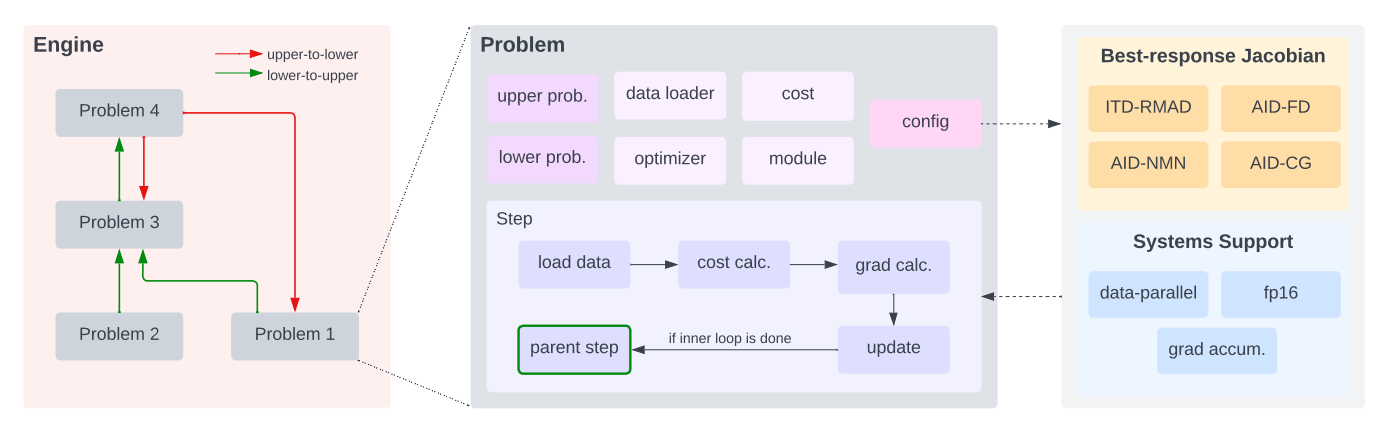
\includegraphics[width=1.0\textwidth]{images/chap4/MLO.png}
    \bicaption{多层级优化策略流程图}{Multi-Level Optimization (MLO) flowchart}
    \label{fig:4-1}
\end{figure}

因此，本章提出了一种多层级优化策略（Multi-Level Optimization，MLO），在多个相互依赖的学习任务之间建立协同优化关系，通过耦合生成模型与分割模型的训练过程，实现数据生成与原子图像分割的端到端联合优化。如图\ref{fig:4-2}所示，该策略由生成数据构建、分割模型训练和性能反馈优化三个层级串联构成：在第一阶段的生成层级中，训练图像到掩膜模型（image-to-mask model）从低质量原子图像中预测掩膜并构建扩展的图像-掩膜样本对，从而有效提升训练数据的规模与多样性；随后在分割层级中，生成样本与原始样本被联合用于分割网络训练，并结合多尺度特征学习增强模型对不同尺度原子结构的表征能力，进而提升分割精度与鲁棒性；最后在反馈层级中，以验证集上的分割性能反向约束生成模型参数更新，持续优化生成掩膜的结构一致性与空间准确性，从而实现生成数据与分割任务之间的有效匹配与协同提升。通过上述多层级优化策略，能够系统地解决原子图像分割中数据不足与模型泛化能力有限的问题，实现高精度的原子定位与结构表征。

\begin{figure} [htb]
    \centering
    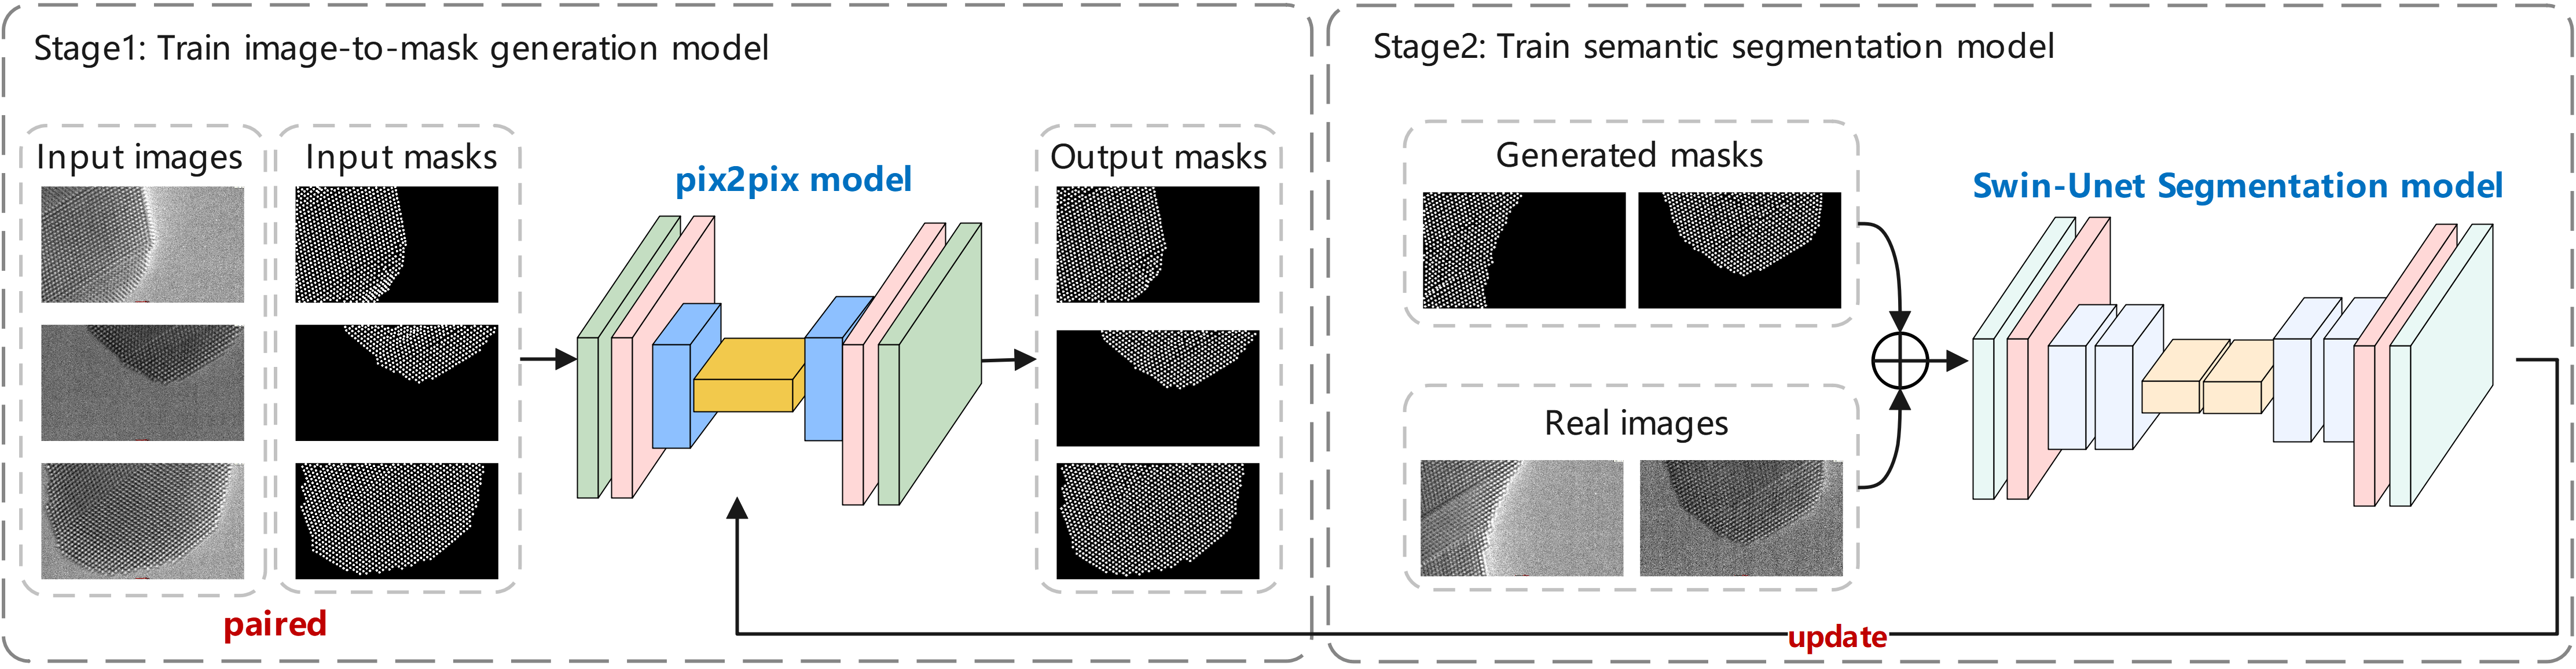
\includegraphics[width=1.0\textwidth]{images/chap4/方法流程图.png}
    \bicaption{方法流程图}{method flowchart}
    \label{fig:4-2}
\end{figure}

\section{基于生成数据增强与多尺度特征融合的原子分割}
这一小节将从生成数据增强策略和多尺度特征融合的原子图像分割方法两个方面，详细介绍所提出的基于多层级优化的原子定位方法的核心技术细节与实现流程。首先，介绍基于图像到掩膜生成的数据增强策略，阐述如何通过条件生成对抗网络实现原子图像到掩膜的映射关系学习，并构建扩展的图像-掩膜样本对以提升训练数据的规模与多样性；随后，介绍基于多尺度特征融合的原子图像分割方法，详细说明如何在swin-transformer中引入多尺度特征融合机制，以增强模型对不同尺度原子结构的表征能力，从而提升分割的精度与鲁棒性。

\subsection{基于图像到掩膜生成的数据增强策略}
针对原子图像标注样本稀缺、低质量成像条件下原子边界模糊以及传统数据增强难以有效扩展结构先验的问题，本章节采用一种基于图像到掩膜生成的数据增强策略。受到Zhang等人\cite{zhang2025generative}采用mask-to-image的方式来扩充医学分割图像工的工作的启发，考虑到本文面向的是原子图像定位场景，其核心需求在于从复杂退化的原子图像中获得可靠的结构标注，因此本文将生成方向由mask-to-image转换为图像到掩膜（image-to-mask），直接利用低质量原子图像生成对应掩膜，以实现伪标注数据构建与训练样本扩充，并进一步服务于后续分割模型的优化。该策略基于条件生成对抗网络，以低质量原子图像和其对应的经过人工标注的高质量掩膜作为输入，学习图像到掩膜的映射关系。设原始训练集记为：

\begin{equation}
\mathcal{D}_{tr}=\{(x_i,y_i)\}_{i=1}^{N},
\end{equation}

其中，$x_i \in \mathbb{R}^{H\times W}$ 表示输入的原子图像，$y_i \in \{0,1\}^{H\times W}$ 表示对应的真实原子掩膜，$N$ 为训练样本数。进一步记验证集为：

\begin{equation}
\mathcal{D}_{val}=\{(x_j^{v},y_j^{v})\}_{j=1}^{M},
\end{equation}

其中，$M$ 为验证样本数。本节的目标是学习一个图像到掩膜生成模型：

\begin{equation}
G_{\phi}: x \rightarrow \hat{y},
\end{equation}
其中，$\phi$ 表示生成模型参数，$\hat{y}=G_{\phi}(x)$ 表示由输入图像预测得到的生成掩膜。基于该模型，可以从原始图像中生成额外的伪标注掩膜，并构造扩展样本对
\begin{equation}
\tilde{\mathcal{D}}_{gen}=\{(x_i,\hat{y}_i)\}_{i=1}^{N}, \qquad \hat{y}_i=G_{\phi}(x_i).
\end{equation}

通过将生成样本与真实标注样本联合使用，可得到增强后的训练集合
\begin{equation}
\mathcal{D}_{aug}=\mathcal{D}_{tr}\cup\tilde{\mathcal{D}}_{gen},
\end{equation}
从而实现训练样本数量与结构多样性的有效扩充。

为实现输入原子图像到目标掩膜之间的映射，本文采用条件生成对抗网络（conditional Generative Adversarial Network, cGAN）构建图像到掩膜生成模型。该模型由生成器 $G_{\phi}$ 和判别器 $D_{\psi}$ 两部分组成，其中生成器负责根据输入图像生成对应掩膜，判别器用于区分真实图像--掩膜对与生成图像--掩膜对。具体而言，生成器学习条件分布
\begin{equation}
p_{\phi}(y|x),
\end{equation}
即在给定输入图像 $x$ 的条件下生成与其对应的掩膜 $y$。

对于真实样本对 $(x,y)$ 和生成样本对 $(x,G_{\phi}(x))$，条件对抗损失可表示为
\begin{equation}
\mathcal{L}_{adv}(G_{\phi},D_{\psi})
=
\mathbb{E}_{(x,y)\sim \mathcal{D}_{tr}}
\left[\log D_{\psi}(x,y)\right]
+
\mathbb{E}_{x\sim \mathcal{D}_{tr}}
\left[\log\left(1-D_{\psi}(x,G_{\phi}(x))\right)\right],
\end{equation}
其中，$\psi$ 为判别器参数。该损失促使生成器输出的掩膜在整体分布上逼近真实标注掩膜。

仅依赖对抗损失难以保证像素级结构精度，因此进一步引入重建损失约束生成掩膜与真实掩膜之间的一致性。本文采用 $L_1$ 重建损失：
\begin{equation}
\mathcal{L}_{rec}(G_{\phi})
=
\mathbb{E}_{(x,y)\sim \mathcal{D}_{tr}}
\left[
\|y-G_{\phi}(x)\|_{1}
\right].
\end{equation}

考虑到原子区域通常面积较小且前景--背景类别分布不均衡，仅采用逐像素重建约束容易导致细粒度结构被背景淹没，因此进一步引入 Dice 损失以增强模型对前景区域与边界信息的刻画能力：
\begin{equation}
\mathcal{L}_{dice}(G_{\phi})
=
1-
\frac{2\sum\limits_{p} G_{\phi}(x)_p y_p+\epsilon}
{\sum\limits_{p} G_{\phi}(x)_p+\sum\limits_{p} y_p+\epsilon},
\end{equation}
其中，$p$ 表示像素位置，$\epsilon$ 为平滑项。

综上，图像到掩膜生成模型的总体优化目标定义为
\begin{equation}
\mathcal{L}_{gen}
=
\lambda_{adv}\mathcal{L}_{adv}
+\lambda_{rec}\mathcal{L}_{rec}
+\lambda_{dice}\mathcal{L}_{dice},
\end{equation}
其中，$\lambda_{adv}$、$\lambda_{rec}$ 和 $\lambda_{dice}$ 分别表示各损失项的权重系数。于是，生成模型的训练过程可表示为
\begin{equation}
\phi^{*}
=
\arg\min_{\phi}\max_{\psi}
\mathcal{L}_{gen}(G_{\phi},D_{\psi}).
\end{equation}

通过上述联合优化，生成器不仅能够学习输入图像与目标掩膜之间的条件映射关系，还能够在对抗判别与像素重建的双重作用下生成具有较好结构一致性和边界准确性的原子掩膜。

在生成模型训练完成后，利用其对训练图像进行逐样本预测，得到对应的掩膜概率图
\begin{equation}
P_i = G_{\phi}(x_i).
\end{equation}
为便于后续构建增强样本，首先对概率图进行阈值化处理，得到二值掩膜
\begin{equation}
\hat{y}_i(p)=
\begin{cases}
1, & P_i(p)\ge \tau,\\
0, & P_i(p)< \tau,
\end{cases}
\end{equation}
其中，$\tau$ 为分割阈值。

由于低质量成像条件下生成结果可能存在局部伪响应、边界断裂或噪声区域，若直接将所有伪标注样本加入训练集，可能会降低增强数据质量。因此，本文进一步引入质量筛选机制，对生成样本进行可靠性评估。定义样本质量函数为
\begin{equation}
q_i = Q(\hat{y}_i),
\end{equation}
其中，$Q(\cdot)$ 用于表征生成掩膜的结构合理性，可根据区域连通性、前景面积比例、平均置信度或边界平滑程度等信息进行构造。当样本满足
\begin{equation}
q_i \ge \eta,
\end{equation}
其中，$\eta$ 为质量阈值，则认为该生成样本具有较高可信度，并保留到有效增强集
\begin{equation}
\tilde{\mathcal{D}}_{eff}
=
\{(x_i,\hat{y}_i)\mid q_i \ge \eta\}.
\end{equation}

最终，用于后续网络训练的增强数据集定义为
\begin{equation}
\mathcal{D}_{eff}=\mathcal{D}_{tr}\cup \tilde{\mathcal{D}}_{eff}.
\end{equation}

该策略的实质在于：利用图像到掩膜生成模型将原本有限的人工标注样本扩展为规模更大、结构分布更丰富的训练样本集合，从而在有限监督条件下提高模型对原子结构的学习能力与泛化能力。

传统的数据增强方法通常将生成过程与下游任务训练过程分开进行，生成模型仅依据重建误差或对抗损失优化，其目标主要在于提高生成结果与真实标注之间的表面相似性。然而，对于原子图像任务而言，生成掩膜是否真正有利于后续分割与定位，并不能仅由像素级相似性来衡量。若生成结果在结构边界、原子响应强度或空间分布上存在偏差，则可能在后续训练中引入噪声监督，削弱增强数据的实际价值。

为此，本文将图像到掩膜生成过程置于多层级优化框架中，并通过下游任务性能反向约束生成模型参数。记后续分割网络参数为 $\theta$，其详细结构将在下一小节中给出。对于给定生成模型参数 $\phi$，分割网络在增强数据集 $\mathcal{D}_{eff}(\phi)$ 上训练后可得到最优参数
\begin{equation}
\theta^{*}(\phi)
=
\arg\min_{\theta}\mathcal{L}_{seg}\big(\theta;\mathcal{D}_{eff}(\phi)\big),
\end{equation}
其中，$\mathcal{L}_{seg}$ 表示分割网络在训练集上的监督损失。

进一步地，在验证集 $\mathcal{D}_{val}$ 上定义外层目标函数
\begin{equation}
\mathcal{L}_{val}\big(\theta^{*}(\phi)\big),
\end{equation}
则生成模型的外层优化目标可写为
\begin{equation}
\phi^{*}
=
\arg\min_{\phi}
\mathcal{L}_{val}\big(\theta^{*}(\phi)\big).
\end{equation}

由此可见，生成模型参数 $\phi$ 不再仅由生成损失 $\mathcal{L}_{gen}$ 决定，而是同时受到验证集分割性能的间接约束。于是，整个图像到掩膜增强过程可视为一个嵌套优化问题：
\begin{equation}
\begin{aligned}
\min_{\phi}\quad & \mathcal{L}_{val}\big(\theta^{*}(\phi)\big) \\
\text{s.t.}\quad 
& \theta^{*}(\phi)=\arg\min_{\theta}\mathcal{L}_{seg}\big(\theta;\mathcal{D}_{eff}(\phi)\big), \\
& \phi=\arg\min_{\phi}\max_{\psi}\mathcal{L}_{gen}(G_{\phi},D_{\psi}).
\end{aligned}
\end{equation}

上述多层级优化机制使得生成模型学习到的不仅是“与真实掩膜相似”的伪标注结果，而且是“有助于提升下游分割性能”的有效增强样本，从而实现生成过程与后续原子定位任务之间的协同优化。


该策略以低质量原子图像为输入，通过条件生成对抗网络学习图像到掩膜的映射关系，自动生成与输入图像相对应的原子掩膜，从而构建扩展的图像--掩膜样本对，为后续分割网络训练提供辅助监督信息。与传统仅依赖几何变换或强度扰动的数据增强方法不同，该方法能够直接从原始图像中学习原子结构与掩膜分布之间的对应关系，使生成结果更符合原子尺度结构表征需求。同时，为避免生成过程与后续分割任务相互割裂，本文进一步将生成模型置于多层级优化框架下，使其参数更新能够受到下游分割性能的反馈约束，从而持续提高生成掩膜的有效性与结构一致性。


\subsection{基于多尺度特征融合的原子图像分割方法}


\section{算法性能验证与实验结果分析}
\subsection{实验数据来源与实验设置}
本章节使用的实验数据主要来源于原位透射电子显微镜实验获得的时间序列图像数据，以及相应的密度泛函理论计算结果。其中，TEM图像序列来自对Au纳米晶在真空及 CO/O$_2$ 反应气氛条件下的原位观测，用于后续的原子结构识别、运动跟踪及应变分析。这些实验数据均已进行人工标注，有像素级的原子位置掩膜，作为分割网络的监督信号。

此外，本章节数据还引入了基于abTEM与ASE的HRTEM物理仿真数据。在设定加速电压、离焦量、像差参数、采样步长等成像条件后，采用冻结声子、多切片传播与CTF成像流程生成模拟图像，并可覆盖碳纳米管、Au FCC晶体Au二十面体纳米颗粒等典型结构。该部分数据用于补充实验样本在结构类型与成像退化条件上的覆盖不足，从而提升分割模型在低信噪比与跨域场景下的鲁棒性和泛化能力。部分实验样本如图\ref{fig:4-3}所示。

\begin{figure} [htb]
    \centering
    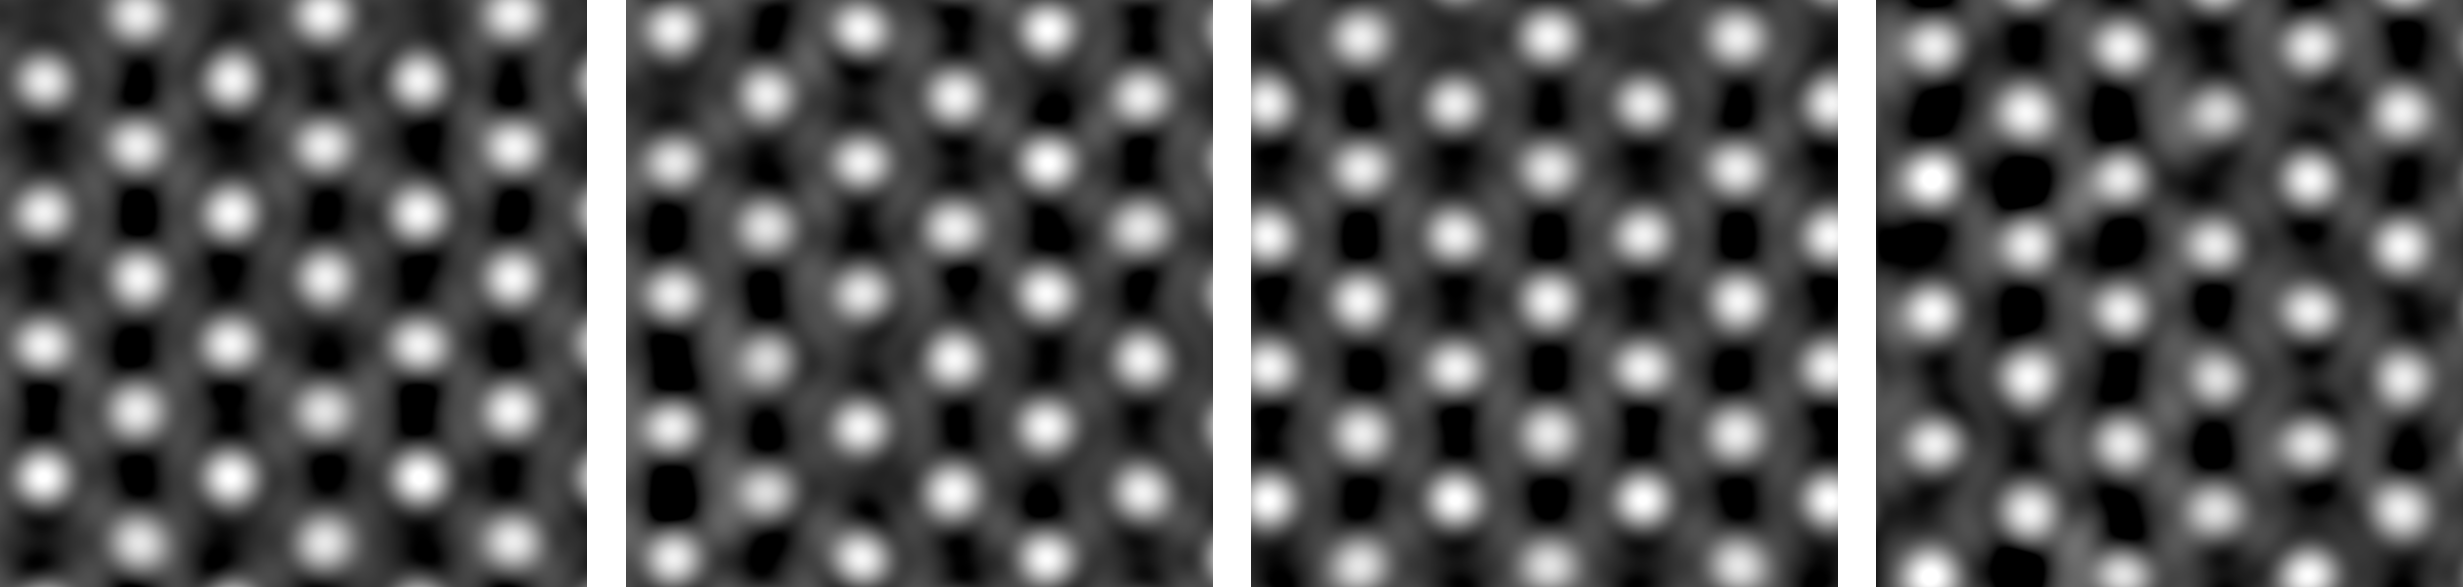
\includegraphics[width=1.0\textwidth]{images/chap4/数据样例.png}
    \bicaption{数据样例图}{data samples}
    \label{fig:4-3}
\end{figure}

实验设置方面，所有模型均在NVIDIA A100 GPU上进行训练与评估。训练过程中采用Adam优化器，初始学习率为0.0002，批量大小为16，训练周期为200个epoch。损失函数的权重系数 $\lambda_{cyc}$、$\lambda_{mask}$、$\lambda_{seg}$ 等通过交叉验证进行调优，以确保生成图像的质量与分割精度之间的平衡。此外，为了评估模型在不同成像条件下的性能，我们设计了多组对比实验，包括单独训练分割网络、仅使用传统CycleGAN进行增强以及引入掩膜加权循环一致性约束的联合优化方法。评估指标方面，分割性能主要通过像素级的准确率（Accuracy）、交并比（IoU）以及边界F1分数（Boundary F1 Score）进行量化评估，而生成图像的质量则通过结构相似性指数（SSIM）和峰值信噪比（PSNR）进行评估。通过上述实验设置，我们能够系统地验证所提出的基于多源特征联合优化的原子定位方法在实际应用中的有效性与优势。


\subsection{实验结果与分析}

\subsection{消融实验与方法有效性验证}


\section{本章小结}


